\chapter{Theoretical Background on EDA}
\label{chap:TheoreticalBackgroundEDA}
\pagestyle{plain}
\vspace{0.5cm}

\noindent This chapter introduces the readers to Electrodermal Activities and how are they related with Music Emotion Recognition task.

\section{Electrodermal phenomena}
Already in the 80's, psychological factors related to electrodermal phenomena were observed. It became an important field of study, due to the fact its ease of obtaining a distinct electrodermal response (EDR), the intensity of which seems apparently related to stimulus intensity and/or its psychological significance \cite{boucsein2012electrodermal}.
\\ \indent
While there is still widespread disagreement and confusion about the nature and causes of musically evoked emotions, recent studies involving real-time observation of brain activity seem to show that areas of the brain linked with emotion (as well as pleasure and reward) are activated by music listening \cite{trost2012mapping}.

\section{Electrodermal Activity}
Electrodermal Activity (EDA) was first introduced by Johnson and Lubin in 1966 \cite{johnson1996} as a common term for all electrical phenomena in skin, including all active and passive electrical properties that can be traced back to the skin and its appendages.
\\
Electrodermal activity (EDA) is the property of the human body that causes continuous variation in the electrical characteristics of the skin. Historically, EDA has also been known as skin conductance, galvanic skin response (GSR), electrodermal response (EDR), psychogalvanic reflex (PGR), skin conductance response (SCR), sympathetic skin response (SSR) and skin conductance level (SCL). The long history of research into the active and passive electrical properties of the skin by a variety of disciplines has resulted in an excess of names, now standardized to electrodermal activity.
\\ \indent
The use of the term \textit{response} for phasic electrodermal phenomena suggests that there is a distinct relationship to a stimulus producing an EDR. Sometimes there are phasic parts that cannot be traced to any specific simulation, they are called \textit{spontaneous} or \textit{non-specific} EDRs.
\\ \indent
There is ample empirical evidence that electrodermal phenomena are generated by sweat gland activity in conjunction with epidermal membrane processes. When sweat gland activity is abolished in humans, either as a result of congenital absence, by sympathectomy, by peripheral sudomotor nerve discharge, or by pharmacological blocking, SCRs and SPRs are normally eliminated and SCL is considerably reduced \cite{fowles1993electrodermal}.
\\ \indent
As mentioned before, skin conductance is characterized by:
\begin{itemize}
	\item Tonic skin conductance level (SCL): smooth underlying slowly changing level, it accounts for the general levels of the coductivity of the skin.
	\item Phasic skin conductance response (SCR): rapidly changing peaks, results from momentary sympathetic activation when arousing stimuli are present.
\end{itemize}
In the figure \ref{fig:signal_phasic} can be seen an EDA file plot and the division in Tonic and Phasic parts thanks to pyphysio library \cite{bizzego2019pyphysio}.
%\begin{figure}[h]
%    \centering
%    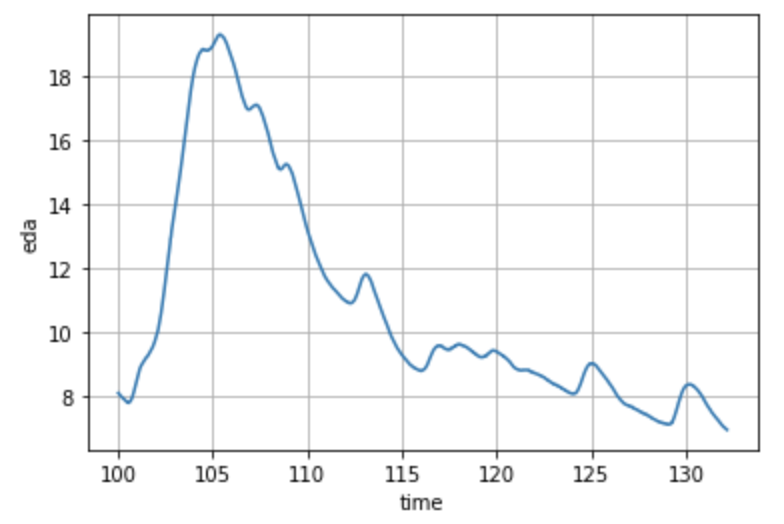
\includegraphics[scale=0.75]{eda_graph.png} 
%	\caption{Graph of an EDA signal plot thanks to \cite{bizzego2019pyphysio} library}
%    \label{fig:eda_graph}
%\end{figure}
\begin{figure}[h]
    \centering
    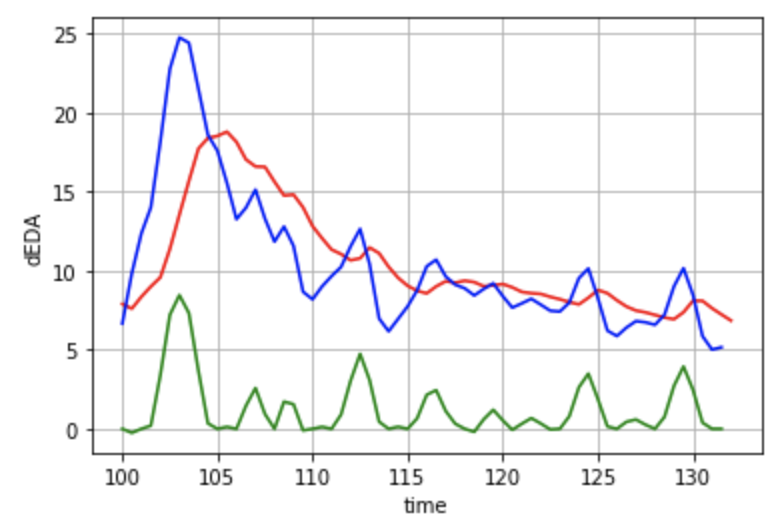
\includegraphics[scale=0.8]{signal_phasic.png} 
	\caption{Representation of EDA signal (in red), driver signal (in blue) and phasic signal (in green)}
    \label{fig:signal_phasic}
\end{figure}
\\
Another useful graph is shown in the figure \ref{fig:phasic_tonic} from \cite{hernandez2014using} that represent division between the complete signal (in blue), the tonic component (in green-dashed) and the phasic component (in red).
\begin{figure}[h]
    \centering
    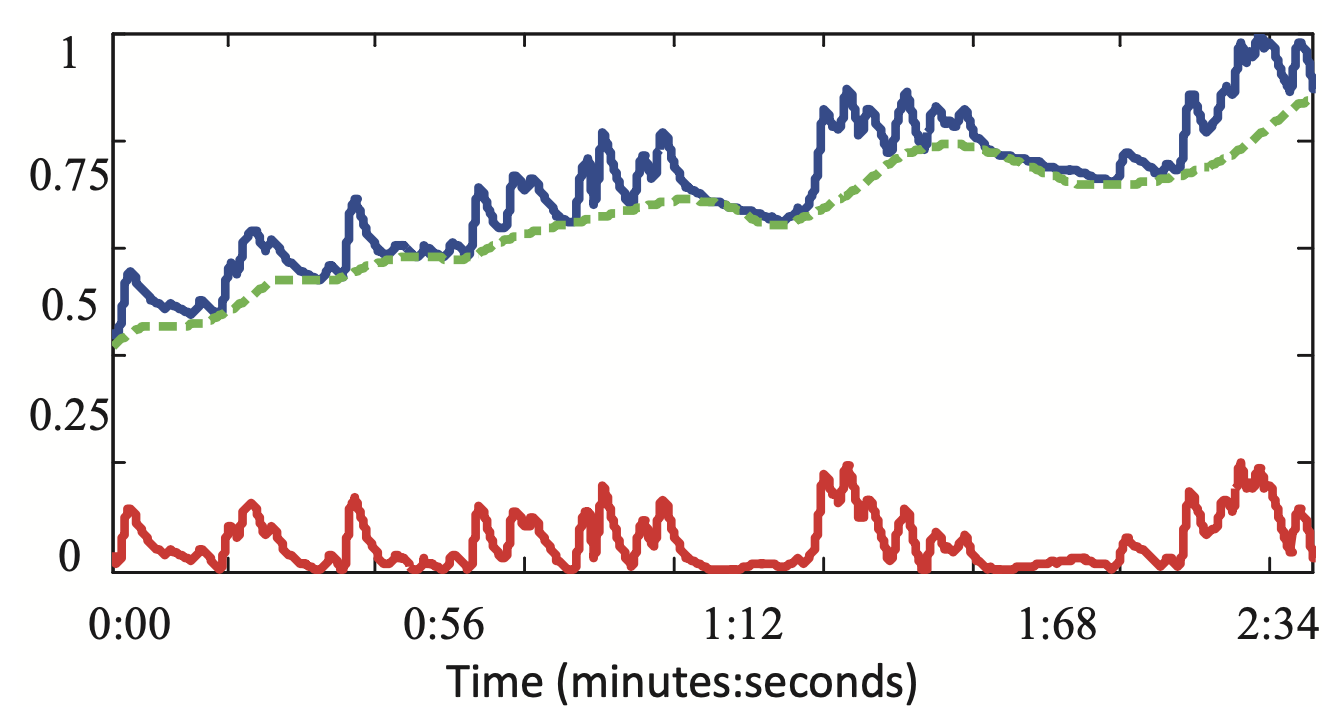
\includegraphics[scale=0.3]{phasic_tonic.png} 
	\caption{Representation of EDA signal (in red), driver signal (in blue) and phasic signal (in green)}
    \label{fig:phasic_tonic}
\end{figure}
\\
The time series of the change of Skin Conductance (SC) can be characterized by a slowly varying tonic activity and fast varying phasic activity. The SCRs shows a steep incline to the peak and a slow decline to the basilne. The successions of SCRs usually results in a superposition of subsequent SCRs as one SCR arises on top of the declining trail of the preceding one.
\\
The figure \ref{fig:skin_conductance} from \cite{benedek2010continuous} shows a SC data section of 165 s, the upper row shows the original SC data. The middle row shows the driver signal which results from deconvolution of the SC data. Inter-impulse data are used to estimate the tonic part of the driver at 10-s intervals (tonic grid points). The tonic driver is used to compute the tonic SC (see upper row). Subtraction of the tonic part from the driver results in the phasic driver (lower row). The phasic driver shows a virtually zero baseline and distinct phasic responses. 
\begin{figure}[h]
    \centering
    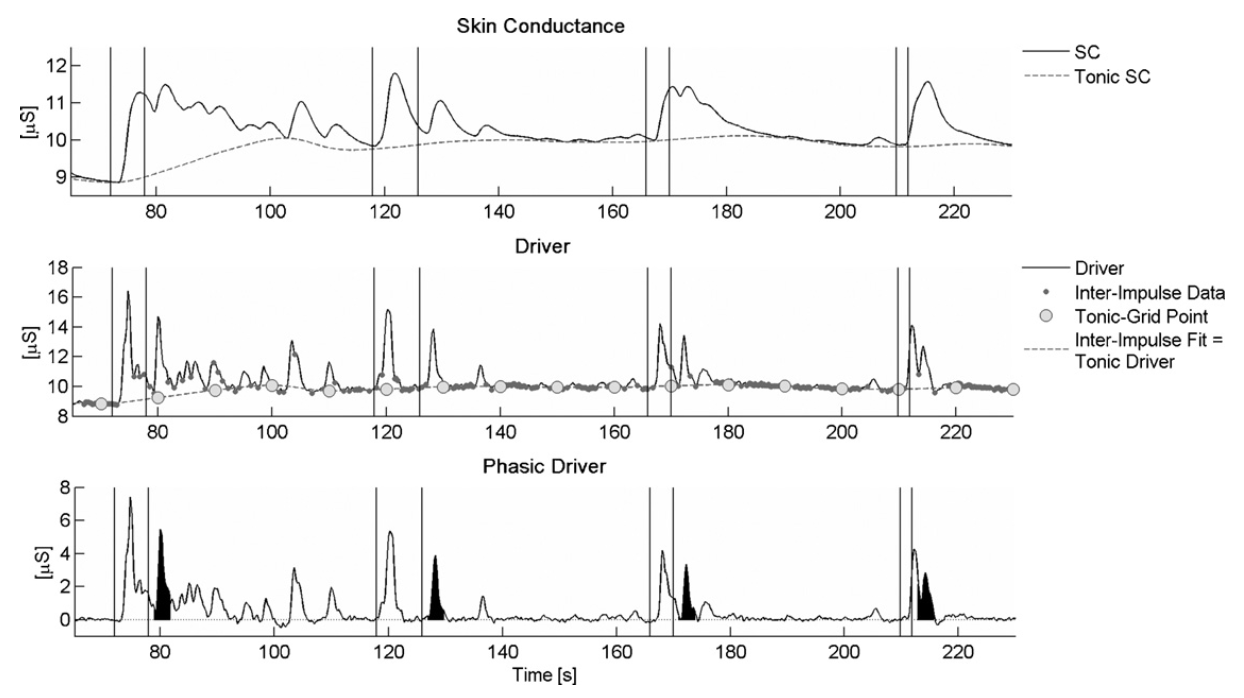
\includegraphics[width=\textwidth]{skin_conductance.png} 
	\caption{Skin conductance and phasic driver extraction}
    \label{fig:skin_conductance}
\end{figure}

\subsection{Measurement principles}
EDA can be measured both without externally applied voltage (endosomatic method) or with application of Direct Current (DC) or Alternating Current (AC) (exosomatic method). The widespread used method is the exosomatic with DC recordings. With direct voltage, skin resistance measurements will result when current is constant, while skin conductance measurement will result when voltage is kept constant.
\\ \indent
There are some factors that should be controlled as possible sources or variance in EDA recordings, like environmental conditions as the climatic conditions and physiological factors like age, gender and ethnic differences.
\\ \indent
EDA can be measured in many different ways electrically including skin potential, resistance, conductance, admittance, and impedance. It achieves this by passing a minuscule amount of current between two electrodes in contact with the skin. The units of measurement for conductance are microSiemens ($\mu$S).

\subsection{Recording techniques}
Electrodermal recording is usually performed with two electrodes. Exosomatic techniques use two active sites, while endosomatic recording requires an active and an inactive site.
\\
Figure \ref{fig:electrode_sites} illustrate the preferred palmar recording areas for exosomatic and endosomatic EDA recordings. Sites A and B for bipolar recordings. C and D for volar electrode sites.
\begin{figure}[h]
    \centering
    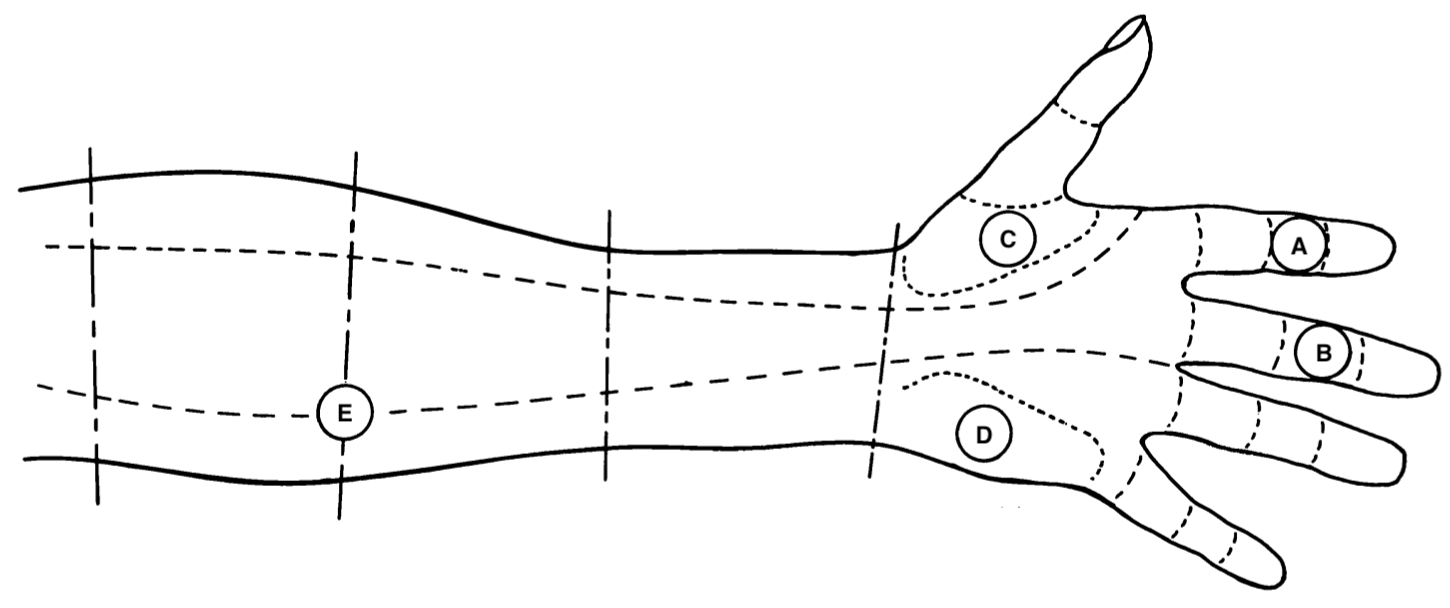
\includegraphics[width=\textwidth]{electrode_sites.png} 
	\caption{Preferred palmar recording areas for exosomatic and endosomatic EDA recordings}
    \label{fig:electrode_sites}
\end{figure}

\subsection{Artifacts identification in EDA data}
EDA data is often captured by wearable devices, which makes the signal collected vulnerable to several types of noise. Artifacts can be generated from electronic noise or variation in the contact between the skin and the recording electrode caused by pressure, excessive movement or adjustment of the device \cite{taylor2015automatic}.
\\
They may be mistaken for a skin conductance response, and this must be avoided.
\\ \indent
Typically, as Boucsein \cite{boucsein2012electrodermal} report, the shape of an SCR typically lasts between $1a$ to $5s$, has a steep onset and an exponentially decay and reaches an amplitude of at least $0.01 \mu S$. An example of a typical SCR in figure \ref{fig:SCR_example}.
\begin{figure}[h]
    \centering
    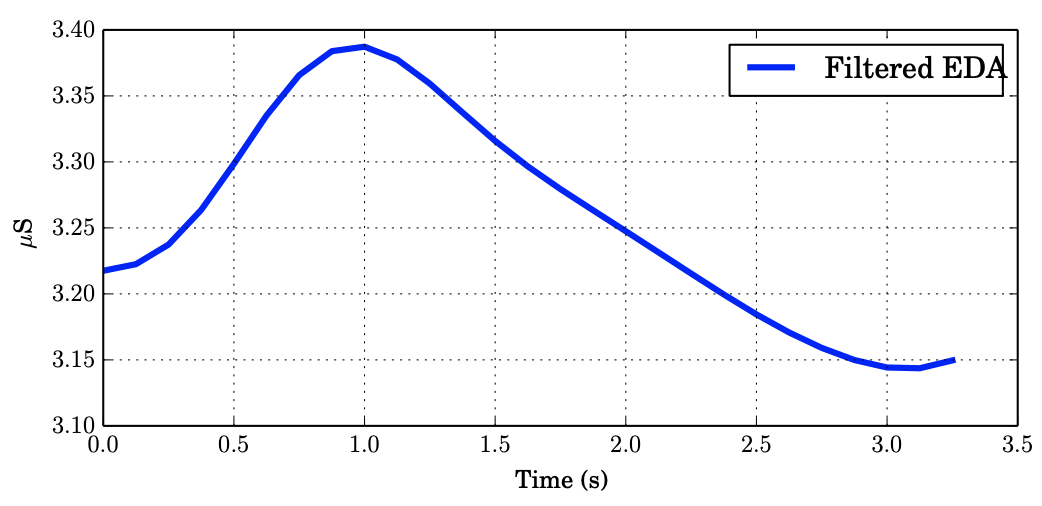
\includegraphics[scale=0.4]{SCR_example.png} 
	\caption{Example of a SCR shape}
    \label{fig:SCR_example}
\end{figure}
\\
Currently, many researchers deal with signal artifacts and noise by applying exponential smoothing or low-pass filtering.
\\
Additionally, filter cutoff frequencies are based only loosely on prior knowledge of typical characteristics of SCR shape, and vary widely study to study (1 and 5 Hz). The cutoff frequency ultimately chosen for a study is specific to that particular study, making generalization difficult.
\\ \indent
There are much relevant techniques that are also able to recognize and compensate for large-magnitude artifacts that can result from pressure or movement of the device during recordings.
\\
In \cite{taylor2015automatic} is presented a figure reported here \ref{fig:eda_artifacts}, which shows a portion of signal that contains three artifacts, in which the fast decrease could not be produced by human physiology. Comparing the raw signal and the filtered version, the low-pass filter has not removed the artifacts.
\begin{figure}[h]
    \centering
    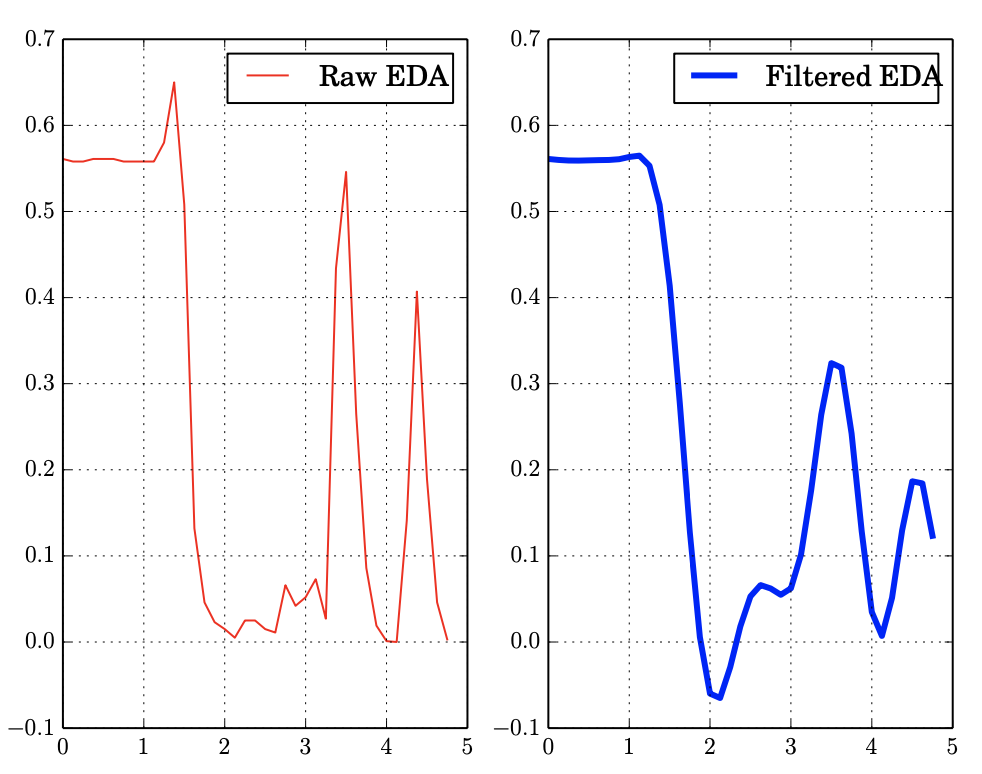
\includegraphics[scale=0.4]{eda_artifacts.png} 
	\caption{Portion of an EDA signal, the raw signal on the left in red, a 1 Hz low-pass filter applied on the signal to the left in blue}
    \label{fig:eda_artifacts}
\end{figure}
\\
Some researchers, as Boucsein analysis \cite{boucsein2012electrodermal}, develop heuristic techniques for removing atypical portion of the EDA signal. Someone decide to discard portion of their data where the signal increased more than 20\% per second or decreased more than 10\% per second.
\\
In another case, a study which collected EDA from two sensors (on both the ankle and wrist) \cite{hedman2010situ} was able to detect artifacts by looking for epochs when only one of the two sensors had an abnormally low signal, or showed an unusually rapid increase or decrease.
\\ \indent
In \cite{taylor2015automatic} developed a Machine Learning algorithm for automatically detecting EDA artifacts, providing empirical evaluation of classification performances.

\subsection{EDA features}
As for MER analysis, also in EDA data analysis, is important to find which features need to be extracted and than which feature selection method must be carried.
\\ \indent
Emotion recognition from EDA has been commonly used for the assessment of user's experience in a variety of contexts such as recreational and games \cite{drachen2010correlation} and driving \cite{healey2005detecting}. Previous research has explored the predictive power of a diverse set of EDA features of different types, including time domain, frequency domain, and time-frequency domain features.
\\ \indent
Regarding time domain features, most usually features considered are the statistical parameters of the signal as:
\begin{itemize}
	\item Mean value: $\mu$ is the central value of a discrete set of numbers $x_1,x_2,...,x_n$, specifically, the sum of the values divided by the number of values:
		\begin{equation}
		\mu=\dfrac{1}{n} \sum_{i=1}^{n}{x_i}
		\end{equation}
	\item Standard deviation:  is a measure of the amount of variation or dispersion of a set of values:
		\begin{equation}
		\sigma=\sqrt{\dfrac{1}{n}\sum_{i=1}^{n}({x_i-\mu})^2}
		\end{equation}
	\item Kurtosis: is a measure of the "tailedness" of the probability distribution of a real-valued random variable:
		\begin{equation}
		kurt=\dfrac{\dfrac{1}{n} \sum_{i=1}^{n}{(x_i-\mu)^4}}{\sigma^4}
		\end{equation}
	\item Skewness: is a measure of the asymmetry of the probability distribution of a real-valued random variable about its mean:
		\begin{equation}
		skew=\dfrac{\dfrac{1}{n} \sum_{i=1}^{n}{(x_i-\mu)^3}}{\sigma^3}
		\end{equation}
\end{itemize}
In \cite{ghaderyan2016efficient}, as an example, were extracted the features for EDA data shown in table .
\begin{table}[h!]
	\centering
	\begin{tabular}{|l |p{0.36\textwidth} | p{0.3\textwidth}|}
		\hline
		Domain & Feature vector & Number of features\\ [0.5ex] 
		\hline\hline Time & SCR related \newline Statistical features \newline Hjorth features \newline Higher Order Crossing & 7 \newline 8 \newline 2 \newline 5 \\ 
		\hline	Frequency	 & Statistical features \newline Band power & 8 \newline 9 \\ 
		\hline	Time-Frequency & DWT coefficients \newline SWT features \newline MFCCs \newline Statistical features MFCC & 56 \newline 40 \newline 481 \newline 5 \\
		\hline
	\end{tabular}
	\caption{Features extracted in \cite{ghaderyan2016efficient}}
	\label{table:browse_music}
\end{table}
Other cases, researchers have focused on event-related features of EDA. They are useful when are presented to the subjects some events, stimulus, like images or sounds.
\\
Examples of event-related aspects of EDA considered in other studies are SCR amplitude, SCR peak count, mean SCR rise time, or the sum of SCR areas.
\\ \indent
Fewer researches, as \cite{shukla2019feature} remarks, fewer researchers has focused on the predictive power of EDA related to the frequency domain. The frequency domain analysis has shown superior capability for the gradient component's detection of individual SCR.
\\
Due to the different rate of physiological process, EDA signals vary significantly with the frequency \cite{ghaderyan2016efficient}.
\\
Frequency oscillations of EDA signals can be divided into different frequency sub-bands to analyze it. Indeed previous researchers has considered statistical aspects.
\\ \indent
As for audio, also for EDA data, after constructing a feature matrix, need to apply an algorithm of feature selection to improve data reliability.
\\ \\
Some examples of feature selection could be:
\begin{itemize}
	\item Joint Mutual Information (JMI): focuses on the increasing complementary information between features.
	\item Conditional Mutual Information Maximization (CMIM): it can properly identify truly redundant features and noisy features, and gives preference to informative, uncorrelated features.
	\item Double Input Symmetrical Relevance (DISR): a normalized variant of JMI.
\end{itemize}
In general it is not known which features are most appropriate for emotion recognition from EDA and previous works have made limited contributions on a systematic comparison of EDA features. 







